
\subsection*{Enemy Turn}

The enemy placement is given by the encounter in the storybook. The order in which enemies are placed cannot be changed without an explicit action allowing you to do so. The seating order is also important, and determines which player gets which enemies. The seating order can be decided by the players.

\subsection*{Enemy Card}
\begin{figure}[ht]
	\begin{minipage}[t][5cm][t]{0.5\textwidth}
		Enemy cards consist of four parts:
		\begin{enumerate}
			\item \textbf{Name}	 - The name of the enemy
			\item \textbf{Passives} - Enemies can have passive effects too
			\item \textbf{Life} - The life total is shown at the top right. When an enemy takes damage, place that many damage markers on that enemy. When the enemy has more damage markers than health, it dies
			\item \textbf{Actions} - enemies have one of two action patterns:\\
			\hspace*{1cm} \textbf{Dice} - Most enemies act according to the \hspace*{1cm} enemy die\\
			\hspace*{0.9cm} \textbf{Rotating} - Some enemies rotate their \hspace*{1cm} actions in a pattern, indicated by letters
		\end{enumerate}
	\end{minipage}	
	\begin{minipage}[t][5cm][t]{0.5\textwidth}
		\centering
		\includegraphics[width=0.9\linewidth, valign=t]{ExplanationPics/Monstercard.drawio.png}
	\end{minipage}
\end{figure}

\subsection*{Enemy actions}
%todo wording
Enemies always attack only the Player in front of them, this means all players can have their enemies act simultaneously.Enemies act sequentially from left to right. 
To perform the enemy turn, look at the monster die,  and have the monster perform the corresponding action.
Repeat once for every enemy.

\begin{figure}[ht]
	\begin{minipage}[t][8cm][t]{1\textwidth}
		\centering
		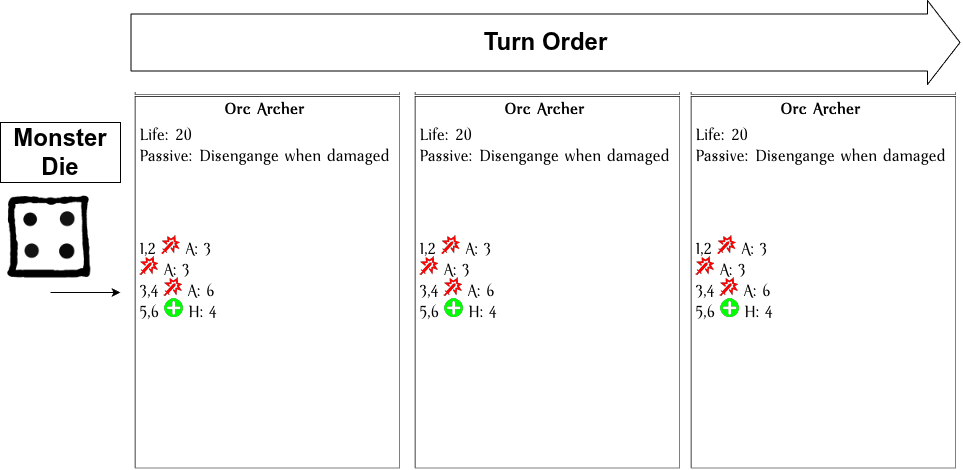
\includegraphics[width=0.9\linewidth, valign=t]{ExplanationPics/MonsterTurn.drawio.png}
	\end{minipage}	
\end{figure}

\textbf{Knocked Out} - If your life reaches 0 while your enemies are still acting, the rest of the enemies still perform their action. No remaining attack hits, but the enemies could still apply boons to themselves or each other, before rotating to the player to your left in the Cleanup step.
